\section{Theorie}
\label{sec:Theorie}

Ein Lock-In-Verstärker ist ein Verstärker mit integriertem phasenempfindlichem Detektor.
Er kann zu Messung stark verrauschter Signale genutzt werden.
Ein schematischer Aufbau ist in Abbildung \autoref{fig:lock_in_amplifier_1} zu sehen:

\begin{figure}[H]
  \centering
  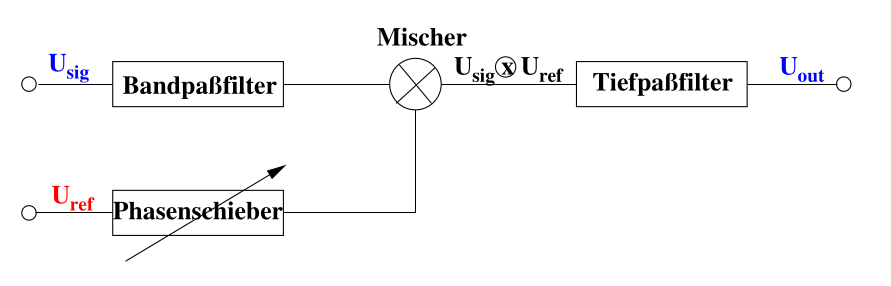
\includegraphics[scale=0.5]{assets/lock_in_amplifier_1.png}
  \caption{Schematischer Aufbau des Lock-In-Verstärkers \cite{V303}}
  \label{fig:lock_in_amplifier_1}
\end{figure}

\noindent Zunächst wird das Nutzsignal $U_\text{Sig}$ mithilfe eines Bandpassfilters gefiltert.\\
Dieser befreit $U_\text{Sig}$ von Frequenzen $\omega \gg \omega_\text{0}$ und $\omega \ll \omega_\text{0}$.
Das Nutzsignal $U_\text{Sig}$ wird darauf von einem Mischer mit einer Referenzspannung Referenzspannung $U_\text{ref}(\omega_\text{0})$ multipliziert.
Die Phasenlage der Referenzspannung kann mit dem Phasenschieber angepasst werden.
Danach wird das Signal durch einen Tiefpassfilter über mehrere Perioden integriert und von möglichen Störungen befreit, sodass am Ausgang eine Spannung
\begin{equation}
  U_\text{out} = \frac{2}{\pi}U_\text{0}\cdot \cos{\left(\phi\right)}
  \label{eqn:Uout}
\end{equation}
gemessen werden kann.
bei einer Phasenverschiebung von 0 ist die Ausgangsspannung maximal und es gilt:
\begin{equation}
  U_\text{out} = \frac{2}{\pi}U_\text{0}
\end{equation}
